\documentclass[UTF8, 12pt]{ctexart}
% UTF8编码,ctexart现实中文
\usepackage{xcolor}
% 使用颜色
\definecolor{orange}{RGB}{255,127,0} 
\definecolor{violet}{RGB}{192,0,255} 
\definecolor{aqua}{RGB}{0,255,255} 
\usepackage{geometry}
\setcounter{tocdepth}{4}
\setcounter{secnumdepth}{4}
% 设置四级目录与标题
\geometry{papersize={21cm,29.7cm}}
% 默认大小为A4
\geometry{left=3.18cm,right=3.18cm,top=2.54cm,bottom=2.54cm}
% 默认页边距为1英尺与1.25英尺
\usepackage{indentfirst}
\setlength{\parindent}{2.45em}
% 首行缩进2个中文字符
\usepackage{amssymb}
% 因为所以与其他数学拓展
\usepackage{amsmath}
% 数学公式
\usepackage[colorlinks,linkcolor=black,urlcolor=blue]{hyperref}
% 超链接
\usepackage{tikz}
% 绘图
\usepackage{setspace}
\renewcommand{\baselinestretch}{1.5}
% 1.5倍行距
\usepackage{pifont}
% 圆圈序号
\usepackage{mathtools}
% 有字的长箭头
\usepackage{yhmath}
% 弧线标识
\usetikzlibrary{decorations.pathreplacing}
% tikz的大括号
\author{Didnelpsun}
\title{微分中值定理与导数的应用}
\date{}
\begin{document}
\maketitle
\pagestyle{empty}
\thispagestyle{empty}
\tableofcontents
\thispagestyle{empty}
\newpage
\pagestyle{plain}
\setcounter{page}{1}

\section{微分中值定理}

三个定理都是建立局部与整体的关系,利用导数控制函数,反之不能使用函数控制导数。

$\text{罗尔定理}\xrightleftharpoons[\text{特例:}f(a)=f(b)]{\text{泛化:任意端点值}}\text{拉格朗日中值定理}\xrightleftharpoons[\text{特例:}F(x)=x]{\text{泛化:参数方程}}\text{柯西中值定理}$

\subsection{罗尔定理}

极值\textcolor{violet}{\textbf{定义:}}若$\exists\delta>0$,使$\forall x\in U(x_0,\delta)$恒有$f(x)\geqslant f(x_0)$,则$f(x)$在$x_0$处取极小值,恒有$f(x)\leqslant f(x_0)$,则$f(x)$在$x_0$处取极大值。

费马引理\textcolor{violet}{\textbf{定义:}}若$f(x)$在$x_0$处取得极值,且$f(x)$在$x_0$处可导,则$f'(x_0)=0$。

罗尔定理\textcolor{violet}{\textbf{定义:}}

\begin{enumerate}
    \item $f(x)$在$[a,b]$上连续。
    \item $f(x)$在$(a,b)$内可导。
    \item $f(a)=f(b)$。
\end{enumerate}

则$\exists\,\xi\in(a,b)$,使得$f'(\xi)=0$。

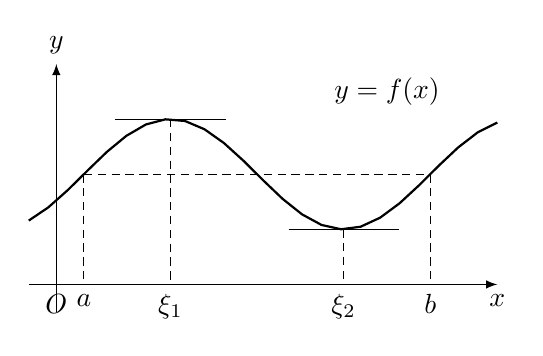
\begin{tikzpicture}[scale=0.7]
    \draw[-latex](-0.5,0) -- (8,0) node[below]{$x$};
    \draw[-latex](0,-0.5) -- (0, 4) node[above]{$y$};
    \filldraw[black] (0,0) node[below]{$O$};
    \draw[black, thick,domain=-0.5:8] plot (\x, {sin((\x-0.5) r)+2});
    \filldraw[black] (6,3.5) node {$y=f(x)$};
    \draw[densely dashed](0.5,2) -- (0.5+2*pi, 2);
    \draw[densely dashed](0.5,2) -- (0.5, 0) node[below]{$a$};
    \draw[densely dashed](0.5+2*pi,2) -- (0.5+2*pi, 0) node[below]{$b$};
    \draw[densely dashed](0.5+pi/2,3) -- (0.5+pi/2, 0) node[below]{$\xi_1$};
    \draw[densely dashed](0.5+pi/2*3,1) -- (0.5+pi/2*3, 0) node[below]{$\xi_2$};
    \draw[black](pi/2-0.5,3) -- (1.5+pi/2,3);
    \draw[black](pi/2*3-0.5,1) -- (1.5+pi/2*3,1);
\end{tikzpicture}

\subsection{拉格朗日中值定理}

\begin{enumerate}
    \item $f(x)$在$[a,b]$上连续。
    \item $f(x)$在$(a,b)$内可导。
\end{enumerate}

则$\exists\,\xi\in(a,b)$,使得$f(b)-f(a)=f'(\xi)(b-a)$。

其中$f(b)-f(a)=f'[a+\theta(b-a)](b-a)(0<\theta<1)$,$\because f'(\xi)=f'[a+(\xi-a)]=f'[a+\dfrac{\xi-a}{b-a}(b-a)]$。\medskip

有限增量公式\textcolor{violet}{\textbf{定义:}}$\Delta y=f(x_0+\Delta x)-f(x_0)=f'[x_0+\theta\Delta x]\Delta x(0<\theta<1)$。

推论:$f(x)$在$I$上连续且可导,则$I$上$f(x)=C\Leftrightarrow f'(x)\equiv 0$

\textbf{例题:}证明$x>0$时,$\dfrac{x}{1+x}<\ln(1+x)<x$。

令$f(x)=\ln x$,又$\ln 1=0$,$\therefore\ln(1+x)=\ln(1+x)-\ln 1$。

根据拉格朗日中值定理$\ln(1+x)-\ln 1=f'(\xi)x=\dfrac{x}{\xi}(1<\xi<1+x)$。

又$\dfrac{x}{1+x}<\dfrac{x}{\xi}<x$,$\therefore$得证。

\subsection{柯西中值定理}

\begin{enumerate}
    \item $f(x)$与$F(x)$在$[a,b]$上连续。
    \item $f(x)$与$F(x)$在$(a,b)$内可导,且$\forall x\in(a,b)$,$F'(x)\neq 0$。
\end{enumerate}

则$\exists\,\xi\in(a,b)$,使得$\dfrac{f(b)-f(a)}{F(b)-F(a)}=\dfrac{f'(\xi)}{F'(\xi)}$。

\section{洛必达法则}

\textcolor{aqua}{\textbf{定理:}}

\begin{enumerate}
    \item 当$x\to a\text{或}\infty$时,函数$f(x)$,$g(x)$都趋向0或无穷大。
    \item $f'(x)$和$F'(x)$在点$a$的某去心邻域内,或$\vert x\vert$大于充分大的正数时,存在,且$g'(x)\neq 0$。
    \item $\lim\limits_{x\to a}\dfrac{f'(x)}{g'(x)}$或$\lim\limits_{x\to\infty}\dfrac{f'(x)}{g'(x)}$存在或无穷大。
    \item $\lim\limits_{x\to a}\dfrac{f(x)}{g(x)}=\lim\limits_{x\to a}\dfrac{f'(x)}{g'(x)}$或$\lim\limits_{x\to\infty}\dfrac{f(x)}{g(x)}=\lim\limits_{x\to\infty}\dfrac{f'(x)}{g'(x)}$。
\end{enumerate}

\textcolor{orange}{注意:}

\begin{enumerate}
    \item 如果函数比值不为$\dfrac{0}{0}$或$\dfrac{\infty}{\infty}$型,则不能使用洛必达法则。
    \item 若求导后极限仍为$\dfrac{0}{0}$或$\dfrac{\infty}{\infty}$型,则可以继续使用洛必达法则。
    \item 若$\lim\limits_{x\to a}\dfrac{f'(x)}{g'(x)}$不存在且不为$\infty$,不能反推$\lim\limits_{x\to a}\dfrac{f(x)}{g(x)}$不存在也不为$\infty$,这时候洛必达法则是失效的。
\end{enumerate}

对于第三个注意点:$\lim\limits_{x\to 0}\dfrac{x^2\cdot\sin\dfrac{1}{x}}{x}=\lim\limits_{x\to 0}x\cdot\sin\dfrac{1}{x}=0$。

而使用洛必达法则:\medskip

$\lim\limits_{x\to 0}\dfrac{x^2\cdot\sin\dfrac{1}{x}}{x}$

$=\lim\limits_{x\to 0}\left(2x\cdot\sin\dfrac{1}{x}-\cos\dfrac{1}{x}\right)$

$=\lim\limits_{x\to 0}\left(-\cos\dfrac{1}{x}\right)=\text{不存在}$

\section{泰勒公式}

非常重要。过去的很多定义如等价无穷小都是基于泰勒公式。

\subsection{定义}

是一个用函数在某点的信息描述其附近取值的公式。如果函数满足一定的条件,泰勒公式可以用函数在某一点的各阶导数值做系数构建一个多项式来近似表达这个函数。即形式:$f(x)=\sum ax^n$。

简单来说,泰勒公式就是一个近似表达函数的公式。其增量趋向0。

对于泰勒公式以及之前的中值定理等相关延申见\href{https://www.zhihu.com/question/25627482}{知乎回答}。

\subsection{泰勒定理}

拉格朗日定理是泰勒定理的特例。泰勒定理也称为泰勒中值定理,与之前的三大中值定理组成四大中值定理,前面的三大中值定理建立函数与一阶导数的关系,而泰勒定理建立函数与高阶导数之间的关系。

\subsubsection{皮亚诺余项}

设$f(x)$在$x_0$处$n$阶可微,则$f(x)=\sum_{k=0}^n\dfrac{f^{(k)}(x_0)}{k!}(x-x_0)^k+o((x-x_0)^n)$。这个就是带皮亚诺余项的泰勒公式。\medskip

$f(x)=\sum_{k=0}^n\dfrac{f^{(k)}(x_0)}{k!}(x-x_0)^k$就是$f(x)$在$x_0$处的$n$次泰勒多项式,$o((x-x_0)^n)$就是函数的皮亚诺余项。

缺点:

\begin{enumerate}
    \item 只给出余项的定性描述,不能进行定量分析。
    \item 适用范围小。
\end{enumerate}

\subsubsection{拉格朗日余项}

设$f(x)$在$x_0$处$n+1$阶可微,$x_0\in I$则$\forall x\in I$,$\exists\,\xi\in I(\xi\in(x_0,x))$使得$f(x)=\sum_{k=0}^n\dfrac{f^{(k)}(x_0)}{k!}(x-x_0)^k+\dfrac{f^{(n+1)}(\xi)}{(n+1)!}(x-x_0)^{n+1}$。这个就是带拉格朗日余项的泰勒公式。

$R_n(x)=\dfrac{f^{(n+1)}(\xi)}{(n+1)!}(x-x_0)^{n+1}$就是函数的拉格朗日余项。

根据拉格朗日中值定理推广的方式:$R_n(x)=\dfrac{f^{(n+1)}[x_0+\theta(x-x_0)]}{(n+1)!}(x-x_0)^{n+1}(\theta\in(0,1))$。

若$\vert f^{(n+1)}(x)\vert\leqslant M$,则$\vert R_n(x)\vert=\dfrac{\vert f^{(n+1)}(\xi)\vert}{(n+1)!}\vert x-x_0\vert^{n+1}\leqslant\dfrac{M}{(n+1)!}\vert x-x_0\vert^{n-1}$。

特点:

\begin{enumerate}
    \item 进行定量研究。
    \item 可以进行整体的研究。
    \item 计算量较大。
\end{enumerate}

\subsection{泰勒展开}

\subsubsection{麦克劳林公式}

当$x_0=0$时$f(x)=f(0)+f'(0)x+\dfrac{f''(0)}{2!}x^2+\cdots+\dfrac{f^{(n)(0)}}{n!}x^n+\text{余项}$为麦克劳林公式:

\begin{enumerate}
    \item $\sin x=x-\dfrac{x^3}{3!}+o(x^3)=(-1)^{n-1}\dfrac{x^{2n-1}}{(2n-1)!}$。
    \item $\cos x=1-\dfrac{x^2}{2!}+\dfrac{x^4}{4!}+o(x^4)=(-1)^n\dfrac{x^{2n}}{(2n)!}$。
    \item $\arcsin x=x+\dfrac{x^3}{3!}+o(x^3)=\dfrac{x^{2n-1}}{(2n-1)!}$。
    \item $\tan x=x+\dfrac{x^3}{3}+o(x^3)$。
    \item $\arctan x=x-\dfrac{x^3}{3}+o(x^3)$。
    \item $\ln(1+x)=x-\dfrac{x^2}{2}+\dfrac{x^3}{3}+o(x^3)=(-1)^n\dfrac{x^n}{n}$。
    \item $e^x=1+x+\dfrac{x^2}{2!}+\dfrac{x^3}{3!}+o(x^3)=\dfrac{x^n}{n!}$。
    \item $(1+x)^\alpha=1+\alpha\cdot x+\dfrac{\alpha\cdot(\alpha-1)}{2!}x^2+o(x^2)$。
\end{enumerate}

其中$o(x^\alpha)$为佩亚诺余项,其非常小。

同样可以对泰勒展开式进行变形:$x-\sin x\sim\dfrac{x^3}{6}$,$x+\sin x\sim 2x$。

如:

$\lim\limits_{x\to 0}\dfrac{[\sin x-\sin(\sin x)]\sin x}{x^4}$

$=\dfrac{\dfrac{1}{6}\sin^3x\cdot\sin x}{x^4}$

$=\dfrac{\dfrac{1}{6}\sin^4x}{x^4}$

$=\dfrac{1}{6}$

\subsubsection{泰勒公式计算}

先写出$y=f(x)$的泰勒公式或麦克劳林公式,再通过比较系数来获得$f^{(n)}(x_0)$:

\begin{enumerate}
    \item 任何一个无穷阶可导的函数(在收敛的情况下)都可以写为: \medskip \\
    $y=f(x)=\sum_{n=0}^\infty\dfrac{f^{(n)}(x_0)}{n!}(x-x_0)^n$ 或 $y=f(x)=\sum_{n=0}^\infty\dfrac{f^{(n)}(0)}{n!}x^n$。
    \item 给出的任意一个具体的无穷阶可导函数$y=f(x)$都可以通过已知的公式展开为幂级数。
    \item 而函数的展开式具有唯一性,比较步骤一步骤二的公式的系数就可以获取倒$f^{(n)}(x_0)$或$f^{(n)}(0)$。
\end{enumerate}

\textbf{例题:}设$y=x^3\sin x$,求$y^{(6)}(0)$。\medskip

\ding{172}$y=\sum_{n=0}^\infty\dfrac{y^{(n)}(0)}{n!}x^n$。\medskip

$\because$需要结果的导数阶数为6,所以最后得到的次数为6就可以了。\medskip

\ding{173}$\therefore y=x^3\left(x-\dfrac{1}{6}x^3+\cdots\right)=x^4-\dfrac{1}{6}x^6+\cdots$(不要写$o(x^n)$,因为这里$x$并不是趋向0的)。

\ding{174}步骤一的抽象函数当$n=6$时为$\dfrac{y^{(6)}(0)}{6!}x^6$,它应该与步骤二得到的$x^4-\dfrac{1}{6}x^6+\cdots$的6阶项的系数相等。

$\therefore \dfrac{y^{(6)}(0)}{6!}=-\dfrac{1}{6}\Rightarrow y^{(6)}(0)=-5!=-120$。

\subsection{展开幂的选择}

泰勒公式展开时应该展开到多少次幂?

\subsubsection{\texorpdfstring{$\dfrac{A}{B}$}\ 型,上下同阶}

当分母或分子式$x$的$k$次幂那么应该把分母或分子展开到对应的次数幂。\medskip

如$\lim\limits_{x\to 0}\dfrac{x-\sin x}{x^3}$展开为三次:\medskip

$\lim\limits_{x\to 0}\dfrac{x-\sin x}{x^3}$

$=\lim\limits_{x\to 0}\dfrac{x-\left[x-\dfrac{1}{6}x^3+o(x^3)\right]}{x^3}$\medskip

$=\lim\limits_{x\to 0}\dfrac{\dfrac{1}{6}x^3+o(x^3)}{x^3}$\medskip

$=\dfrac{1}{6}$

\subsubsection{\texorpdfstring{$A-B$}\ 型,幂次最低}

将$A$,$B$分别展到他们系数不相等的$x$的最低次幂为止。

如已知当$x\to 0$时,$\cos x-e^{-\frac{x^2}{2}}$与$ax^k$为等价无穷小,求$a$,$b$。

泰勒展开:

$
\begin{aligned}
    & \cos x-e^{-\frac{x^2}{2}} \\
    & = 1-\dfrac{x^2}{2}+\dfrac{1}{24}x^4+o(x^4)-\left(1-\dfrac{x^2}{2}+\dfrac{1}{8}x^4+o(x^4)\right) \\
    & = -\dfrac{1}{12}x^4+o(x^4) \\
    & \sim -\dfrac{1}{12}x^4
\end{aligned}
$

$\therefore a=-\dfrac{1}{12},b=4$。

\textbf{例题:}求解$\lim\limits_{x\to 0}\dfrac{\sin^2x-x^2}{e^{x^4}-1}$。

首先由泰勒展开式$e^x=1+x+o(x)$,得到$e^x-1\sim x$。

$\therefore e^{x^4}-1\sim x^4$。

然后泰勒展开:

$x-\sin x$

$= 1\cdot x^1+0\cdot x^3 - (1\cdot x^1-\dfrac{1}{6}x^3+o(x^3))$

$= \dfrac{1}{6}x^3+o(x^3)$

$\sim \dfrac{1}{6}x^3$

$x+\sin x$

$=x-(-\sin x)$

$=1\cdot x^1-(-1\cdot x^1)+o(x)$

$=2x+o(x)$

$\sim 2x$

$\therefore$

$\lim\limits_{x\to 0}\dfrac{\sin^2x-x^2}{e^{x^4}-1}$\medskip

$=\lim\limits_{x\to 0}\dfrac{(\sin x+x)(\sin x-x)}{x^4}$\medskip

$=\lim\limits_{x\to 0}\dfrac{2x\cdot\left(-\dfrac{1}{6}x^3\right)}{x^4}$\medskip

$=-\dfrac{1}{3}$

\section{函数单调性与曲线凹凸性}

\subsection{函数单调性}

\textcolor{aqua}{\textbf{定理:}}

\begin{enumerate}
    \item 函数$f(x)$在区间$[a,b]$上连续,在$(a,b)$内可导。
    \item 若$(a,b)$内$f'(x)\geqslant 0$,且等号只有有限个点上成立,则$f(x)$在$[a,b]$上单调增加。
    \item 若$(a,b)$内$f'(x)\leqslant 0$,且等号只有有限个点上成立,则$f(x)$在$[a,b]$上单调减少。
\end{enumerate}

\textbf{例题:}证明$x>0$时,$x-\dfrac{x^3}{6}<\sin x<x$。

首先令$f(x)=x-\sin x$,而$f(0)=0$。

$f'(x)=1-\cos x\geqslant 0$,则$f(x)$在$R$上递增。

$\therefore$在$(0,+\infty]$上$f(x)>f(0)=0$,即$x>\sin x$。

令$g(x)=\sin x-x-\dfrac{x^3}{6}$,而$g(0)=0$。

$g'(x)=\cos x-1+\dfrac{x^2}{2}\geqslant 0$,则$g(x)$在$R$上递增。

$\therefore$在$(0,+\infty]$上$g(x)>g(0)=0$,即$\sin x>x-\dfrac{x^3}{6}$。

得证。

\subsection{曲线凹凸性与拐点}

\textcolor{violet}{\textbf{定义:}}若函数$f(x)$在区间$I$上连续,且对$I$上任意两点$x_1,x_2$恒有:

\begin{enumerate}
    \item $f(\dfrac{x_1+x_2}{2})<\dfrac{f(x_1)+f(x_2)}{2}$,则$f(x)$在$I$上凹。
    \item $f(\dfrac{x_1+x_2}{2})>\dfrac{f(x_1)+f(x_2)}{2}$,则$f(x)$在$I$上凸。
\end{enumerate}

而当凹凸性发生改变的点就是拐点。

\textcolor{aqua}{\textbf{定理:}}

\begin{enumerate}
    \item 函数$f(x)$在区间$[a,b]$上连续,在$(a,b)$内二阶可导。
    \item 若$(a,b)$内$f''(x)>0$,则$f(x)$在$[a,b]$上凹。
    \item 若$(a,b)$内$f'(x)<0$,则$f(x)$在$[a,b]$上凸。
\end{enumerate}

拐点的二阶导数等于0,或拐点在二阶导数不存在的点。

\textbf{例题:}证明凹凸性与二阶导数的关系。

不妨先证明凹函数与二阶导数的关系。已知$f''(x)>0$

不妨设$x_1<x_2$,且$\dfrac{x_1+x_2}{2}=x_0$。

$f(x_1)+f(x_2)-2(x_0)$

$=[f(x_2)-f(x_0)]-[f(x_1)-f(x_0)]$

$\xRightarrow{\text{拉格朗日中值定理}}$

$=f'(\xi_2)(x_2-x_0)-f'(\xi_1)(x_0-x_1)$

$=\dfrac{x_2-x_1}{2}[f'(\xi_2)-f'(\xi_1)]>0$

$\therefore f''(x)>0\Rightarrow f(\dfrac{x_1+x_2}{2})<\dfrac{f(x_1)+f(x_2)}{2}$。

\section{函数极值与最值}

\subsection{函数极值}

极值\textcolor{violet}{\textbf{定义:}}若$\exists\,\delta>0$,使

$\forall x\in U(x_0,\delta)$恒有$f(x)\geqslant f(x_0)$,则$f(x)$在$x_0$取极小值。

$\forall x\in U(x_0,\delta)$恒有$f(x)\leqslant f(x_0)$,则$f(x)$在$x_0$取极大值。

\textcolor{aqua}{\textbf{定理:}}(极值必要条件)

若$f(x)$在$x_0$处可导,且$x_0$处取得极值,则$f'(x_0)=0$。

\textcolor{aqua}{\textbf{定理:}}(极值第一充分条件)

设$f(x)$在$\mathring{U}(x_0,\delta)$内可导,且$f'(x_0)=0$或在$x_0$连续。

\begin{enumerate}
    \item 若$x<x_0$时,$f'(x)\geqslant 0$,$x>x_0$时$f'(x)\leqslant 0$,则$x_0$取得极大值。
    \item 若$x>x_0$时,$f'(x)\geqslant 0$,$x<x_0$时$f'(x)\leqslant 0$,则$x_0$取得极小值。
    \item 若$f'(x)$在$x_0$处不变号,则无极值点。
\end{enumerate}

\textcolor{aqua}{\textbf{定理:}}(极值第二充分条件)

若$f'(x_0)=0$而且$f''(x_0)\neq 0$:

\begin{enumerate}
    \item 当$f''(x_0)<0$,则$f(x)$在$x_0$取极大值。
    \item 当$f''(x_0)>0$,则$f(x)$在$x_0$取极小值。
\end{enumerate}

\subsection{函数最值}

\subsubsection{连续函数闭区间最值}

\begin{enumerate}
    \item 求出$f(x)$在$(a,b)$内的驻点和不可导的点$x_1,x_2\cdots,x_n$。
    \item 求出函数值$f(x_1),f(x_2)\cdots,f(x_n)$与端点值$f(a),f(b)$。
    \item 比较求出最值。
\end{enumerate}

\subsubsection{最值应用题}

\begin{enumerate}
    \item 建立目标函数并确定定义域。
    \item 求出驻点并计算值。
\end{enumerate}

\section{函数图像绘制}

\subsection{基本步骤}

\begin{enumerate}
    \item 确定函数定义域,并考察其奇偶性与周期性。
    \item 求出一阶导数与二阶导数,并计算导数为0与不存在的点。
    \item 根据导数判断增减性与凹凸性,并求出极值与拐点。
    \item 求出渐近线。
    \item 确定另外的特殊点。
\end{enumerate}

\subsection{函数渐近线}

\begin{itemize}
    \item 若$\lim\limits_{x\to\infty}f(x)=A$,那么$y=A$就是水平渐近线。
    \item 若$\lim\limits_{x\to x_0}f(x)=\infty$,那么$x=x_0$就是垂直渐近线。
    \item 若$\lim\limits_{x\to\infty}\dfrac{f(x)}{x}=a,b=\lim\limits_{x\to\infty}(f(x)-ax)$,那么$y=ax+b$就是斜渐近线。
\end{itemize}

\section{弧微分与曲率}

\subsection{弧微分}

\begin{minipage}{0.5\linewidth}
    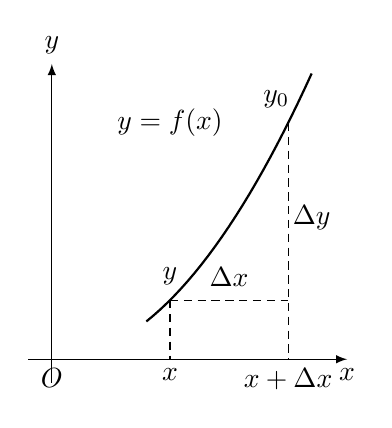
\begin{tikzpicture}[scale=3]
        \draw[-latex](-0.1,0) -- (1.25,0) node[below]{$x$};
        \draw[-latex](0,-0.1) -- (0,1.25) node[above]{$y$};
        \filldraw[black] (0,0) node[below]{$O$};
        \draw[black, thick,domain=0.4:1.1] plot (\x, \x*\x);
        \filldraw[black] (0.5,1) node {$y=f(x)$};
        \draw[densely dashed](0.5,0.25) -- (0.5, 0) node[below]{$x$};
        \draw[densely dashed](1,1) -- (1, 0) node[below]{$x+\Delta x$};
        \draw[densely dashed](0.5,0.25) -- (1,0.25);
        \filldraw[black](0.5,0.35) node{$y$};
        \filldraw[black](0.95,1.1) node{$y_0$};
        \filldraw[black](0.75,0.35) node{$\Delta x$};
        \filldraw[black](1.1,0.6) node{$\Delta y$};
    \end{tikzpicture} 
\end{minipage}
\hfill
\begin{minipage}{0.4\linewidth}
    $\vert\wideparen{yy_0}\vert=S(x)$

    $\Delta y=f(x+\Delta x)-f(x)$

    $(\Delta s)^2\approx(\Delta x)^2+(\Delta y)^2$
\end{minipage}\medskip

当偏移量无穷小时,$y=f(x)$所构成的线段就是一条直线,所以:

\begin{minipage}{0.5\linewidth}
    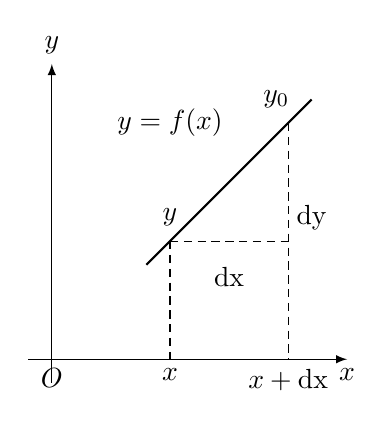
\begin{tikzpicture}[scale=3]
        \draw[-latex](-0.1,0) -- (1.25,0) node[below]{$x$};
        \draw[-latex](0,-0.1) -- (0,1.25) node[above]{$y$};
        \filldraw[black] (0,0) node[below]{$O$};
        \draw[black, thick,domain=0.4:1.1] plot (\x, \x);
        \filldraw[black] (0.5,1) node {$y=f(x)$};
        \draw[densely dashed](0.5,0.5) -- (0.5, 0) node[below]{$x$};
        \draw[densely dashed](1,1) -- (1, 0) node[below]{$x+\rm{d} x$};
        \draw[densely dashed](0.5,0.5) -- (1,0.5);
        \filldraw[black](0.5,0.6) node{$y$};
        \filldraw[black](0.95,1.1) node{$y_0$};
        \filldraw[black](0.75,0.35) node{$\rm{d} x$};
        \filldraw[black](1.1,0.6) node{$\rm{d} y$};
    \end{tikzpicture} 
\end{minipage}
\hfill
\begin{minipage}{0.4\linewidth}
    $\rm{d} y=f(x+\rm{d} x)-f(x)$

    $(\rm{d} s)^2=(\rm{d} x)^2+(\rm{d} y)^2$

    $\rm{d}s=\sqrt{(\rm{d}x)^2+(\rm{d}y)^2}$(弧微分)
\end{minipage}

对于弧微分:

\begin{itemize}
    \item 若直角坐标系下$y=f(x)$,$\rm{d}s=\sqrt{1+\left(\dfrac{\rm{d}y}{\rm{d}x}\right)^2}\rm{d}x$$=\sqrt{1+f'^2(x)}\rm{d}x$,即$\rm{d}s=$$\sqrt{1+f'^2(x)}\rm{d}x$。
    \item 若参数方程下:$x=\phi(t),y=\psi(t)$,$\rm{d}s=\sqrt{\left(\dfrac{\rm{d}x}{\rm{d}t}\right)^2+\left(\dfrac{\rm{d}y}{\rm{d}t}\right)^2}\rm{d}t$\medskip\\$=\sqrt{\psi'^2(t)+\phi'^2(t)}\rm{d}t$,即$\rm{d}s=\sqrt{\psi'^2(t)+\phi'^2(t)}\rm{d}t$。
\end{itemize}

\subsection{曲率与曲率半径}

曲率\textcolor{violet}{\textbf{定义:}}表明曲线在某一点的弯曲程度的数值,针对曲线上某个点的切线方向角对弧长的转动率,通过微分来定义,表明曲线偏离直线的程度。曲率越大,表示曲线的弯曲程度越大。

曲率的倒数就是曲率半径。\medskip

\begin{minipage}{0.5\linewidth}
    两点切线改变角相同时,弯曲程度与两点之间的弧长度成反比。

    两点之间的弧长度相同时,弯曲程度与两点切线改变角成正比。
\end{minipage}
\hfill
\begin{minipage}{0.2\linewidth}
    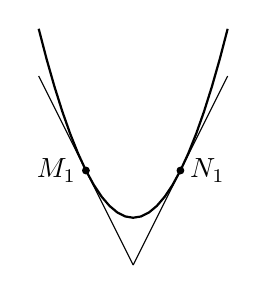
\begin{tikzpicture}[scale=0.6]
        \draw[black, thick,domain=-2:2] plot (\x, {\x*\x});
        \filldraw[black] (-1,1) circle (2pt) node[left]{$M_1$};
        \filldraw[black] (1,1) circle (2pt) node[right]{$N_1$};
        \draw[black](2,3) -- (0,-1);
        \draw[black](-2,3) -- (0,-1);
    \end{tikzpicture}
\end{minipage}
\hfill
\begin{minipage}{0.2\linewidth}
    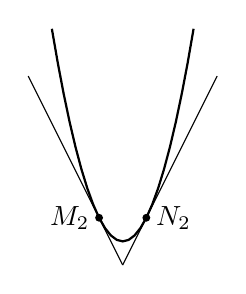
\begin{tikzpicture}[scale=0.6]
        \draw[black, thick,domain=-1.5:1.5] plot (\x, {2*\x*\x});
        \filldraw[black] (-1/2,1/2) circle (2pt) node[left]{$M_2$};
        \filldraw[black] (1/2,1/2) circle (2pt) node[right]{$N_2$};
        \draw[black](2,3.5) -- (0,-1/2);
        \draw[black](-2,3.5) -- (0,-1/2);
    \end{tikzpicture}
\end{minipage}

\begin{minipage}{0.3\linewidth}
    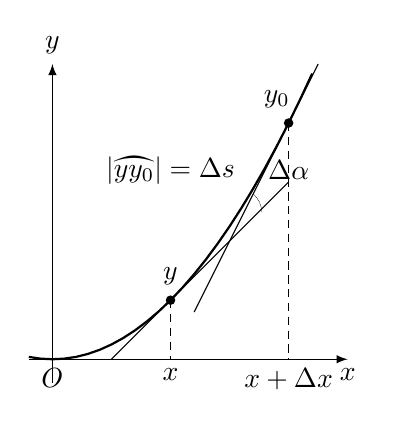
\begin{tikzpicture}[scale=3]
        \draw[-latex](-0.1,0) -- (1.25,0) node[below]{$x$};
        \draw[-latex](0,-0.1) -- (0,1.25) node[above]{$y$};
        \filldraw[black] (0,0) node[below]{$O$};
        \draw[black, thick,domain=-0.1:1.1] plot (\x, \x*\x);
        \draw[densely dashed](0.5,0.25) -- (0.5, 0) node[below]{$x$};
        \draw[densely dashed](1,1) -- (1, 0) node[below]{$x+\Delta x$}; 
        \filldraw[black](0.5,0.35) node{$y$};
        \filldraw[black](0.95,1.1) node{$y_0$};
        \filldraw[black] (1/2,1/4) circle (0.5pt);
        \filldraw[black] (1,1) circle (0.5pt);
        \draw[black](1,3/4) -- (1/4,0);
        \draw[black](0.6,0.2) -- (9/8,5/4);
        \draw[line width=0.1] (0.85,0.7) arc (50:0:0.1);
        \filldraw[black](1,0.8) node{$\Delta\alpha$};
        \filldraw[black](0.5,0.8) node{$\vert\wideparen{yy_0}\vert=\Delta s$};
    \end{tikzpicture} 
\end{minipage}
\hfill
\begin{minipage}{0.6\linewidth}
    $y-y_0$平均曲率:$\hat{k}=\dfrac{\vert\Delta\alpha\vert}{\vert\Delta s\vert}$。\medskip

    $y$曲率:$k=\lim\limits_{\Delta x\to 0}\left\lvert\dfrac{\Delta\alpha}{\Delta s}\right\rvert=\left\lvert\dfrac{\rm{d}\alpha}{\rm{d}s}\right\rvert$($\alpha$为$y$处切线与$x$轴所成角)。
\end{minipage}\medskip

需要对曲率公式进行化简,得到$s$与$\alpha$关于$x$的表示。根据弧微分的定义:$\rm{d}s=$$\sqrt{1+f'^2(x)}\rm{d}x$。

而对于$\alpha$:$\tan\alpha=y'=f'(x)$。

两边对$x$求导:$\sec^2\alpha\cdot\dfrac{\rm{d}\alpha}{\rm{d}x}=y''=f''(x)$。

又$\because\sec^2\alpha=1+\tan^2\alpha=1+y'^2$。

$\therefore\dfrac{\rm{d}\alpha}{\rm{d}x}=\dfrac{y''}{1+y'^2}\Rightarrow\rm{d}\alpha=\dfrac{y''}{1+y'^2}\rm{d}x$。

$\therefore k=\left\lvert\dfrac{\rm{d}\alpha}{\rm{d}s}\right\rvert=\dfrac{\vert y''\vert}{(1+y'^2)^{\frac{3}{2}}}$。


\begin{minipage}{0.5\linewidth}
    $\bigcirc O$为函数$L$在点$X$处的曲率圆,该圆与$L$在$X$处相切,切线为$T$。

    该点的曲率半径为$R$,其中$R=\dfrac{1}{K}$。
\end{minipage}
\hfill
\begin{minipage}{0.4\linewidth}
    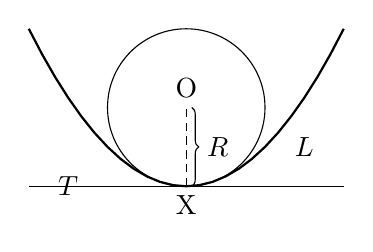
\begin{tikzpicture}[scale=2]
        \draw (-1,0) -- (1,0);
        \node (X) at (0,0)[below]{X};
        \node (O) at (0,0.5)[above]{O};
        \draw[densely dashed] (X) -- (O);
        \filldraw[black] (0.75,0.25) node{$L$};
        \draw[decorate,decoration={brace,mirror,raise=2pt}] (X) -- (O);
        \filldraw[black] (0.2,0.25) node{$R$};
        \filldraw[black] (-0.75,0) node{$T$};
        \draw[black, thick,domain=-1:1] plot (\x, \x*\x);
        \draw[black] (0,0.5) circle (0.5);
    \end{tikzpicture} 
\end{minipage}

\end{document}
